\documentclass[]{article}
\usepackage{lmodern}
\usepackage{amssymb,amsmath}
\usepackage{ifxetex,ifluatex}
\usepackage{fixltx2e} % provides \textsubscript
\ifnum 0\ifxetex 1\fi\ifluatex 1\fi=0 % if pdftex
  \usepackage[T1]{fontenc}
  \usepackage[utf8]{inputenc}
\else % if luatex or xelatex
  \ifxetex
    \usepackage{mathspec}
  \else
    \usepackage{fontspec}
  \fi
  \defaultfontfeatures{Ligatures=TeX,Scale=MatchLowercase}
\fi
% use upquote if available, for straight quotes in verbatim environments
\IfFileExists{upquote.sty}{\usepackage{upquote}}{}
% use microtype if available
\IfFileExists{microtype.sty}{%
\usepackage{microtype}
\UseMicrotypeSet[protrusion]{basicmath} % disable protrusion for tt fonts
}{}
\usepackage[margin=1in]{geometry}
\usepackage{hyperref}
\hypersetup{unicode=true,
            pdftitle={Assignment 1},
            pdfborder={0 0 0},
            breaklinks=true}
\urlstyle{same}  % don't use monospace font for urls
\usepackage{color}
\usepackage{fancyvrb}
\newcommand{\VerbBar}{|}
\newcommand{\VERB}{\Verb[commandchars=\\\{\}]}
\DefineVerbatimEnvironment{Highlighting}{Verbatim}{commandchars=\\\{\}}
% Add ',fontsize=\small' for more characters per line
\usepackage{framed}
\definecolor{shadecolor}{RGB}{248,248,248}
\newenvironment{Shaded}{\begin{snugshade}}{\end{snugshade}}
\newcommand{\AlertTok}[1]{\textcolor[rgb]{0.94,0.16,0.16}{#1}}
\newcommand{\AnnotationTok}[1]{\textcolor[rgb]{0.56,0.35,0.01}{\textbf{\textit{#1}}}}
\newcommand{\AttributeTok}[1]{\textcolor[rgb]{0.77,0.63,0.00}{#1}}
\newcommand{\BaseNTok}[1]{\textcolor[rgb]{0.00,0.00,0.81}{#1}}
\newcommand{\BuiltInTok}[1]{#1}
\newcommand{\CharTok}[1]{\textcolor[rgb]{0.31,0.60,0.02}{#1}}
\newcommand{\CommentTok}[1]{\textcolor[rgb]{0.56,0.35,0.01}{\textit{#1}}}
\newcommand{\CommentVarTok}[1]{\textcolor[rgb]{0.56,0.35,0.01}{\textbf{\textit{#1}}}}
\newcommand{\ConstantTok}[1]{\textcolor[rgb]{0.00,0.00,0.00}{#1}}
\newcommand{\ControlFlowTok}[1]{\textcolor[rgb]{0.13,0.29,0.53}{\textbf{#1}}}
\newcommand{\DataTypeTok}[1]{\textcolor[rgb]{0.13,0.29,0.53}{#1}}
\newcommand{\DecValTok}[1]{\textcolor[rgb]{0.00,0.00,0.81}{#1}}
\newcommand{\DocumentationTok}[1]{\textcolor[rgb]{0.56,0.35,0.01}{\textbf{\textit{#1}}}}
\newcommand{\ErrorTok}[1]{\textcolor[rgb]{0.64,0.00,0.00}{\textbf{#1}}}
\newcommand{\ExtensionTok}[1]{#1}
\newcommand{\FloatTok}[1]{\textcolor[rgb]{0.00,0.00,0.81}{#1}}
\newcommand{\FunctionTok}[1]{\textcolor[rgb]{0.00,0.00,0.00}{#1}}
\newcommand{\ImportTok}[1]{#1}
\newcommand{\InformationTok}[1]{\textcolor[rgb]{0.56,0.35,0.01}{\textbf{\textit{#1}}}}
\newcommand{\KeywordTok}[1]{\textcolor[rgb]{0.13,0.29,0.53}{\textbf{#1}}}
\newcommand{\NormalTok}[1]{#1}
\newcommand{\OperatorTok}[1]{\textcolor[rgb]{0.81,0.36,0.00}{\textbf{#1}}}
\newcommand{\OtherTok}[1]{\textcolor[rgb]{0.56,0.35,0.01}{#1}}
\newcommand{\PreprocessorTok}[1]{\textcolor[rgb]{0.56,0.35,0.01}{\textit{#1}}}
\newcommand{\RegionMarkerTok}[1]{#1}
\newcommand{\SpecialCharTok}[1]{\textcolor[rgb]{0.00,0.00,0.00}{#1}}
\newcommand{\SpecialStringTok}[1]{\textcolor[rgb]{0.31,0.60,0.02}{#1}}
\newcommand{\StringTok}[1]{\textcolor[rgb]{0.31,0.60,0.02}{#1}}
\newcommand{\VariableTok}[1]{\textcolor[rgb]{0.00,0.00,0.00}{#1}}
\newcommand{\VerbatimStringTok}[1]{\textcolor[rgb]{0.31,0.60,0.02}{#1}}
\newcommand{\WarningTok}[1]{\textcolor[rgb]{0.56,0.35,0.01}{\textbf{\textit{#1}}}}
\usepackage{graphicx,grffile}
\makeatletter
\def\maxwidth{\ifdim\Gin@nat@width>\linewidth\linewidth\else\Gin@nat@width\fi}
\def\maxheight{\ifdim\Gin@nat@height>\textheight\textheight\else\Gin@nat@height\fi}
\makeatother
% Scale images if necessary, so that they will not overflow the page
% margins by default, and it is still possible to overwrite the defaults
% using explicit options in \includegraphics[width, height, ...]{}
\setkeys{Gin}{width=\maxwidth,height=\maxheight,keepaspectratio}
\IfFileExists{parskip.sty}{%
\usepackage{parskip}
}{% else
\setlength{\parindent}{0pt}
\setlength{\parskip}{6pt plus 2pt minus 1pt}
}
\setlength{\emergencystretch}{3em}  % prevent overfull lines
\providecommand{\tightlist}{%
  \setlength{\itemsep}{0pt}\setlength{\parskip}{0pt}}
\setcounter{secnumdepth}{0}
% Redefines (sub)paragraphs to behave more like sections
\ifx\paragraph\undefined\else
\let\oldparagraph\paragraph
\renewcommand{\paragraph}[1]{\oldparagraph{#1}\mbox{}}
\fi
\ifx\subparagraph\undefined\else
\let\oldsubparagraph\subparagraph
\renewcommand{\subparagraph}[1]{\oldsubparagraph{#1}\mbox{}}
\fi

%%% Use protect on footnotes to avoid problems with footnotes in titles
\let\rmarkdownfootnote\footnote%
\def\footnote{\protect\rmarkdownfootnote}

%%% Change title format to be more compact
\usepackage{titling}

% Create subtitle command for use in maketitle
\newcommand{\subtitle}[1]{
  \posttitle{
    \begin{center}\large#1\end{center}
    }
}

\setlength{\droptitle}{-2em}

  \title{Assignment 1}
    \pretitle{\vspace{\droptitle}\centering\huge}
  \posttitle{\par}
    \author{}
    \preauthor{}\postauthor{}
    \date{}
    \predate{}\postdate{}
  

\begin{document}
\maketitle

\begin{Shaded}
\begin{Highlighting}[]
\KeywordTok{library}\NormalTok{(tidyverse) }\CommentTok{# essential tools}
\KeywordTok{library}\NormalTok{(ggdendro)}
\end{Highlighting}
\end{Shaded}

\hypertarget{question-1}{%
\section{Question 1}\label{question-1}}

For the dataset given, do these calculations by hand:

\begin{itemize}
\tightlist
\item
  Calculate a distance matrix using squared euclidean distance.
\item
  Use hierarchical clustering with single linkage to cluster the data.
  Draw the dendro- gram and identify the two-cluster solution.
\item
  Use hierarchical clustering with average linkage to cluster the data.
  Draw the den- drogram and identify the two-cluster solution.
\item
  Cluster the data using kmeans with k = 2. Use starting clusters of
  (a,b,c) and (d,e).
\end{itemize}

\begin{Shaded}
\begin{Highlighting}[]
\KeywordTok{set.seed}\NormalTok{(}\DecValTok{123}\NormalTok{)}
\CommentTok{# Generating data}
\NormalTok{x <-}\StringTok{ }\KeywordTok{matrix}\NormalTok{(}\KeywordTok{sample}\NormalTok{(}\OperatorTok{-}\DecValTok{5}\OperatorTok{:}\DecValTok{5}\NormalTok{, }\DecValTok{10}\NormalTok{), }\DataTypeTok{nrow =} \DecValTok{5}\NormalTok{)}
\KeywordTok{rownames}\NormalTok{(x) <-}\StringTok{ }\NormalTok{letters[}\DecValTok{1}\OperatorTok{:}\DecValTok{5}\NormalTok{]}
\KeywordTok{colnames}\NormalTok{(x) <-}\StringTok{ }\KeywordTok{c}\NormalTok{(}\StringTok{"U"}\NormalTok{, }\StringTok{"V"}\NormalTok{)}
\NormalTok{x}
\end{Highlighting}
\end{Shaded}

\begin{verbatim}
##    U  V
## a -2 -5
## b  2 -3
## c  5  3
## d  4 -4
## e  1  0
\end{verbatim}

\begin{Shaded}
\begin{Highlighting}[]
\NormalTok{dx <-}\StringTok{ }\KeywordTok{dist}\NormalTok{(x)}\OperatorTok{^}\DecValTok{2} \CommentTok{# finding distances}
\NormalTok{dx}
\end{Highlighting}
\end{Shaded}

\begin{verbatim}
##     a   b   c   d
## b  20            
## c 113  45        
## d  37   5  50    
## e  34  10  25  25
\end{verbatim}

\begin{Shaded}
\begin{Highlighting}[]
\CommentTok{# building  clusters}
\NormalTok{hs <-}\StringTok{ }\KeywordTok{hclust}\NormalTok{(dx, }\StringTok{"single"}\NormalTok{)}
\NormalTok{ha <-}\StringTok{ }\KeywordTok{hclust}\NormalTok{(dx, }\StringTok{"average"}\NormalTok{)}


\CommentTok{# ggplot version }
\KeywordTok{ggdendrogram}\NormalTok{(}\KeywordTok{as.dendrogram}\NormalTok{(hs))}
\end{Highlighting}
\end{Shaded}

\begin{center}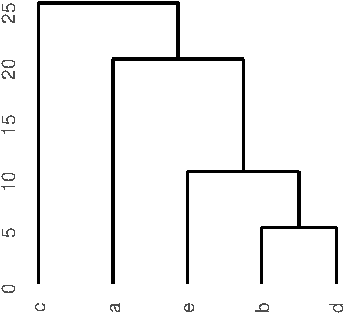
\includegraphics{sol_A1_files/figure-latex/unnamed-chunk-2-1} \end{center}

\begin{Shaded}
\begin{Highlighting}[]
\KeywordTok{ggdendrogram}\NormalTok{(}\KeywordTok{as.dendrogram}\NormalTok{(ha))}
\end{Highlighting}
\end{Shaded}

\begin{center}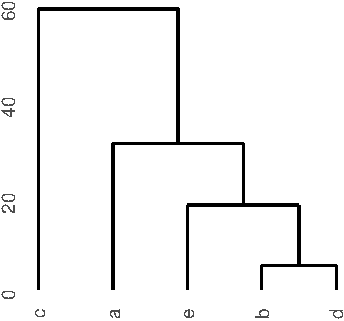
\includegraphics{sol_A1_files/figure-latex/unnamed-chunk-2-2} \end{center}

\begin{Shaded}
\begin{Highlighting}[]
\NormalTok{c1 <-}\StringTok{ }\KeywordTok{apply}\NormalTok{(x[}\DecValTok{1}\OperatorTok{:}\DecValTok{3}\NormalTok{,], }\DecValTok{2}\NormalTok{, mean)}
\NormalTok{c2 <-}\StringTok{ }\KeywordTok{apply}\NormalTok{(x[}\DecValTok{4}\OperatorTok{:}\DecValTok{5}\NormalTok{,], }\DecValTok{2}\NormalTok{, mean)}


\KeywordTok{kmeans}\NormalTok{(x, }\DataTypeTok{centers =} \KeywordTok{rbind}\NormalTok{(c1, c2), }\DataTypeTok{algorithm =} \StringTok{"Lloyd"}\NormalTok{)}
\end{Highlighting}
\end{Shaded}

\begin{verbatim}
## K-means clustering with 2 clusters of sizes 2, 3
## 
## Cluster means:
##           U         V
## 1 -0.500000 -2.500000
## 2  3.666667 -1.333333
## 
## Clustering vector:
## a b c d e 
## 1 2 2 2 1 
## 
## Within cluster sum of squares by cluster:
## [1] 17.00000 33.33333
##  (between_SS / total_SS =  30.9 %)
## 
## Available components:
## 
## [1] "cluster"      "centers"      "totss"        "withinss"    
## [5] "tot.withinss" "betweenss"    "size"         "iter"        
## [9] "ifault"
\end{verbatim}

\begin{Shaded}
\begin{Highlighting}[]
\NormalTok{x }\OperatorTok\StringTok{ }
\StringTok{  }\KeywordTok{as.data.frame}\NormalTok{() }\OperatorTok\StringTok{ }
\StringTok{  }\KeywordTok{ggplot}\NormalTok{(}\KeywordTok{aes}\NormalTok{(U, V)) }\OperatorTok{+}
\StringTok{  }\KeywordTok{geom_point}\NormalTok{(}\DataTypeTok{colour =} \StringTok{"orange"}\NormalTok{, }\DataTypeTok{size =} \DecValTok{2}\NormalTok{) }\OperatorTok{+}
\StringTok{  }\KeywordTok{theme_bw}\NormalTok{()}
\end{Highlighting}
\end{Shaded}

\begin{center}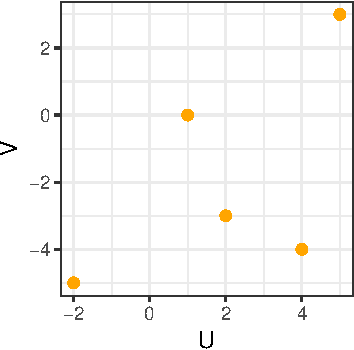
\includegraphics{sol_A1_files/figure-latex/unnamed-chunk-2-3} \end{center}

\hypertarget{question-2}{%
\section{Question 2}\label{question-2}}

Eight online shoppers buy 8, 11, 7 , 6, 5, 6 , 7, 8 pairs of socks. The
same eight shoppers buy 0, 0, 0, 0, 1, 1, 1, 1 computers.

\begin{enumerate}
\def\labelenumi{\alph{enumi})}
\tightlist
\item
  If you run kmeans on this data with \(k = 2\), with no scaling, what
  result would you expect?
\end{enumerate}

\begin{Shaded}
\begin{Highlighting}[]
\NormalTok{my_df <-}\StringTok{ }\KeywordTok{data.frame}\NormalTok{(}\DataTypeTok{x =} \KeywordTok{c}\NormalTok{(}\DecValTok{8}\NormalTok{, }\DecValTok{11}\NormalTok{, }\DecValTok{7}\NormalTok{, }\DecValTok{6}\NormalTok{, }\DecValTok{5}\NormalTok{, }\DecValTok{6}\NormalTok{, }\DecValTok{7}\NormalTok{, }\DecValTok{8}\NormalTok{), }
                 \DataTypeTok{y =} \KeywordTok{c}\NormalTok{(}\DecValTok{0}\NormalTok{, }\DecValTok{0}\NormalTok{, }\DecValTok{0}\NormalTok{,}\DecValTok{0}\NormalTok{, }\DecValTok{1}\NormalTok{, }\DecValTok{1}\NormalTok{, }\DecValTok{1}\NormalTok{, }\DecValTok{1}\NormalTok{))}

\NormalTok{my_df }\OperatorTok\StringTok{ }
\KeywordTok{ggplot}\NormalTok{(}\KeywordTok{aes}\NormalTok{(x, }\KeywordTok{factor}\NormalTok{(y))) }\OperatorTok{+}
\StringTok{  }\KeywordTok{geom_point}\NormalTok{(}\DataTypeTok{colour =} \StringTok{"orange"}\NormalTok{, }\DataTypeTok{size =} \DecValTok{2}\NormalTok{) }\OperatorTok{+}
\StringTok{  }\KeywordTok{theme_bw}\NormalTok{() }\OperatorTok{+}
\StringTok{  }\KeywordTok{geom_text}\NormalTok{(}\DataTypeTok{label =} \DecValTok{1}\OperatorTok{:}\DecValTok{8}\NormalTok{,}\DataTypeTok{hjust=} \FloatTok{-0.7}\NormalTok{, }\DataTypeTok{vjust =} \FloatTok{0.3}\NormalTok{) }\OperatorTok{+}
\StringTok{  }\KeywordTok{labs}\NormalTok{(}\DataTypeTok{y =} \StringTok{'y'}\NormalTok{)}
\end{Highlighting}
\end{Shaded}

\begin{center}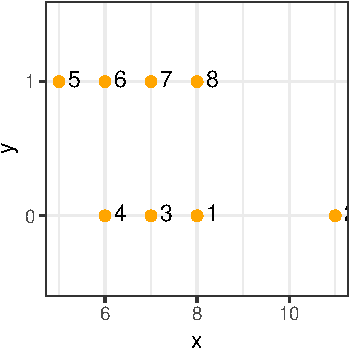
\includegraphics{sol_A1_files/figure-latex/unnamed-chunk-3-1} \end{center}

\begin{Shaded}
\begin{Highlighting}[]
\KeywordTok{kmeans}\NormalTok{(my_df, }\DecValTok{2}\NormalTok{)}\OperatorTok{$}\NormalTok{cluster}
\end{Highlighting}
\end{Shaded}

\begin{verbatim}
## [1] 1 1 2 2 2 2 2 1
\end{verbatim}

\begin{Shaded}
\begin{Highlighting}[]
\KeywordTok{kmeans}\NormalTok{(my_df, }\DecValTok{2}\NormalTok{, }\DataTypeTok{nstart =} \DecValTok{10}\NormalTok{)}\OperatorTok{$}\NormalTok{cluster}
\end{Highlighting}
\end{Shaded}

\begin{verbatim}
## [1] 2 1 2 2 2 2 2 2
\end{verbatim}

NOTE: use nstart to run the algorithm from 10 random starts. Better
convergence. Point 2 is in a cluster of its own!

\begin{enumerate}
\def\labelenumi{\alph{enumi})}
\setcounter{enumi}{1}
\tightlist
\item
  If both variables are scaled to unit standard deviation, what will
  kmeans with \(k = 2\) give you?
\end{enumerate}

\begin{Shaded}
\begin{Highlighting}[]
\NormalTok{d1 <-}\StringTok{ }\NormalTok{my_df }\OperatorTok\StringTok{ }
\StringTok{  }\KeywordTok{mutate_all}\NormalTok{(scale, }\DataTypeTok{center =} \OtherTok{FALSE}\NormalTok{)}

\NormalTok{d1 }\OperatorTok\StringTok{ }
\KeywordTok{ggplot}\NormalTok{(}\KeywordTok{aes}\NormalTok{(x, y)) }\OperatorTok{+}
\StringTok{  }\KeywordTok{geom_point}\NormalTok{(}\DataTypeTok{colour =} \StringTok{"orange"}\NormalTok{, }\DataTypeTok{size =} \DecValTok{2}\NormalTok{) }\OperatorTok{+}
\StringTok{  }\KeywordTok{theme_bw}\NormalTok{() }\OperatorTok{+}
\StringTok{  }\KeywordTok{geom_text}\NormalTok{(}\DataTypeTok{label =} \DecValTok{1}\OperatorTok{:}\DecValTok{8}\NormalTok{,}\DataTypeTok{hjust=} \FloatTok{-0.7}\NormalTok{, }\DataTypeTok{vjust =} \FloatTok{0.3}\NormalTok{) }\OperatorTok{+}
\StringTok{  }\KeywordTok{labs}\NormalTok{(}\DataTypeTok{y =} \StringTok{'y'}\NormalTok{)}
\end{Highlighting}
\end{Shaded}

\begin{center}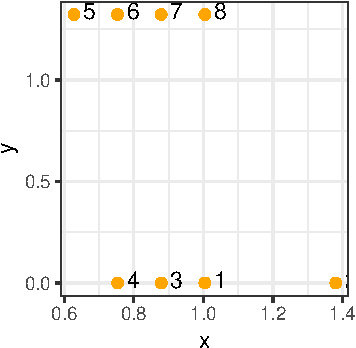
\includegraphics{sol_A1_files/figure-latex/unnamed-chunk-4-1} \end{center}

\begin{Shaded}
\begin{Highlighting}[]
\KeywordTok{kmeans}\NormalTok{(d1, }\DecValTok{2}\NormalTok{, }\DataTypeTok{nstart =} \DecValTok{10}\NormalTok{)}
\end{Highlighting}
\end{Shaded}

\begin{verbatim}
## K-means clustering with 2 clusters of sizes 4, 4
## 
## Cluster means:
##           x        y
## 1 0.8161517 1.322876
## 2 1.0044944 0.000000
## 
## Clustering vector:
## [1] 2 2 2 2 1 1 1 1
## 
## Within cluster sum of squares by cluster:
## [1] 0.07882883 0.22072072
##  (between_SS / total_SS =  92.3 %)
## 
## Available components:
## 
## [1] "cluster"      "centers"      "totss"        "withinss"    
## [5] "tot.withinss" "betweenss"    "size"         "iter"        
## [9] "ifault"
\end{verbatim}

Points 1-4 in 1 cluster, 5-8 in the other.

\begin{enumerate}
\def\labelenumi{\alph{enumi})}
\setcounter{enumi}{2}
\tightlist
\item
  Suppose socks cost 2 euro and the computer is 2000 euro. What is you
  clustered the amount spent by each customer using kmeans with
  \(k = 2\), with no scaling?
\end{enumerate}

\begin{Shaded}
\begin{Highlighting}[]
\NormalTok{d <-}\StringTok{ }\NormalTok{my_df }\OperatorTok\StringTok{ }
\StringTok{  }\KeywordTok{mutate}\NormalTok{(}\DataTypeTok{x =} \DecValTok{2}\OperatorTok{*}\NormalTok{x, }\DataTypeTok{y =} \DecValTok{2000}\OperatorTok{*}\NormalTok{y)}

\NormalTok{d }\OperatorTok\StringTok{ }
\KeywordTok{ggplot}\NormalTok{(}\KeywordTok{aes}\NormalTok{(x, y)) }\OperatorTok{+}
\StringTok{  }\KeywordTok{geom_point}\NormalTok{(}\DataTypeTok{colour =} \StringTok{"orange"}\NormalTok{, }\DataTypeTok{size =} \DecValTok{2}\NormalTok{) }\OperatorTok{+}
\StringTok{  }\KeywordTok{theme_bw}\NormalTok{() }\OperatorTok{+}
\StringTok{  }\KeywordTok{geom_text}\NormalTok{(}\DataTypeTok{label =} \DecValTok{1}\OperatorTok{:}\DecValTok{8}\NormalTok{,}\DataTypeTok{hjust=} \FloatTok{-0.7}\NormalTok{, }\DataTypeTok{vjust =} \FloatTok{0.3}\NormalTok{) }\OperatorTok{+}
\StringTok{  }\KeywordTok{labs}\NormalTok{(}\DataTypeTok{y =} \StringTok{'y'}\NormalTok{)}
\end{Highlighting}
\end{Shaded}

\begin{center}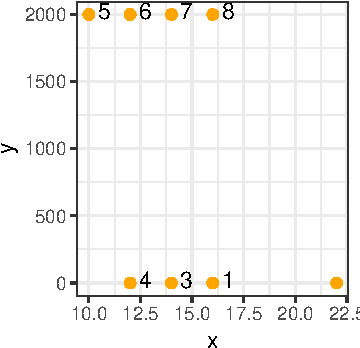
\includegraphics{sol_A1_files/figure-latex/unnamed-chunk-5-1} \end{center}

\begin{Shaded}
\begin{Highlighting}[]
\KeywordTok{kmeans}\NormalTok{(d, }\DecValTok{2}\NormalTok{, }\DataTypeTok{nstart =} \DecValTok{10}\NormalTok{)}
\end{Highlighting}
\end{Shaded}

\begin{verbatim}
## K-means clustering with 2 clusters of sizes 4, 4
## 
## Cluster means:
##    x    y
## 1 13 2000
## 2 16    0
## 
## Clustering vector:
## [1] 2 2 2 2 1 1 1 1
## 
## Within cluster sum of squares by cluster:
## [1] 20 56
##  (between_SS / total_SS = 100.0 %)
## 
## Available components:
## 
## [1] "cluster"      "centers"      "totss"        "withinss"    
## [5] "tot.withinss" "betweenss"    "size"         "iter"        
## [9] "ifault"
\end{verbatim}

Points 1-4 in 1 cluster, 5-8 in the other.

\hypertarget{question-3}{%
\section{Question 3}\label{question-3}}

The file \texttt{eupop.txt} contains the population and percentage
distribution by age for EU countries in 1999. The age categories are
0-14 years, 15-44 years, 45-64 years and 65 years and over.

\begin{enumerate}
\def\labelenumi{\alph{enumi})}
\tightlist
\item
  Construct the euclidean distance matrix of the percentage variables.
  Use it to cluster the countries, using average linkage. Draw the
  dendrogram and interpret. Are there any outlier countries?
\end{enumerate}

\begin{Shaded}
\begin{Highlighting}[]
\NormalTok{eupop <-}\StringTok{ }\KeywordTok{read.table}\NormalTok{(}\StringTok{"data/eupop.txt"}\NormalTok{) }\OperatorTok\StringTok{ }
\StringTok{  }\KeywordTok{select}\NormalTok{(}\OperatorTok{-}\DecValTok{5}\NormalTok{)}
\NormalTok{d <-}\StringTok{ }\KeywordTok{dist}\NormalTok{(eupop)}
\NormalTok{h <-}\StringTok{ }\KeywordTok{hclust}\NormalTok{(d, }\StringTok{"average"}\NormalTok{)}
\KeywordTok{ggdendrogram}\NormalTok{(}\KeywordTok{as.dendrogram}\NormalTok{(h))}
\end{Highlighting}
\end{Shaded}

\begin{center}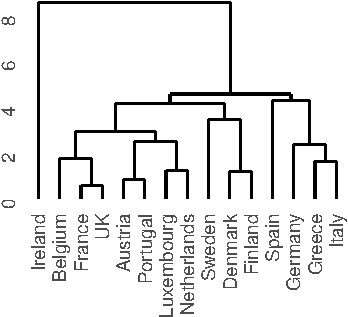
\includegraphics{sol_A1_files/figure-latex/unnamed-chunk-6-1} \end{center}

Ireland is an outlier.

\begin{enumerate}
\def\labelenumi{\alph{enumi})}
\setcounter{enumi}{1}
\tightlist
\item
  Examine the 3-cluster solution. Which countries belong to each of the
  three clusters? Summarise the partitions with sumPartition (in
  h1code.R) Interpret your findings.
\end{enumerate}

\begin{Shaded}
\begin{Highlighting}[]
\KeywordTok{source}\NormalTok{(}\StringTok{'code/h1code.R'}\NormalTok{)}
\KeywordTok{sumPartition}\NormalTok{(eupop, }\KeywordTok{cutree}\NormalTok{(h,}\DecValTok{3}\NormalTok{))}
\end{Highlighting}
\end{Shaded}

\begin{verbatim}
## Final Partition
## 
## Number of clusters  3
## 
##           N.obs Within.clus.SS Ave.dist..Centroid Max.dist.centroid
## Cluster 1    10         55.305           2.211730          4.030199
## Cluster 2     4         17.535           1.831295          3.117090
## Cluster 3     1          0.000           0.000000          0.000000
## 
## 
## Cluster centroids
## 
##       Cluster 1 Cluster 2 Cluster 3 Grand centrd
## p014  18.23     15.25     22.2      17.7        
## p1544 42.52     43.775    46.2      43.1        
## p4564 23.94     24.25     20.3      23.78       
## p65.  15.36     16.725    11.3      15.45333    
## 
## 
## Distances between Cluster centroids
## 
##           Cluster 1 Cluster 2 Cluster 3
## Cluster 1  0.000000  3.523457  7.683521
## Cluster 2  3.523457  0.000000  9.960735
## Cluster 3  7.683521  9.960735  0.000000
\end{verbatim}

Ireland is in Cluster 3. Germany Greece, Italy, Spain are in Cluster 2.
Everyone else is in Cluster 1. Cluster 3: highest proportion of
children(under 15), lowest percentage of over 65. Cluster 2: below
average for under 15s and above average proportion of over 65s. Cluster
2 and 3 are furtherest apart, cluster 1 and 2 are closest. Cluster 2 is
more compact than cluster 1.

\begin{enumerate}
\def\labelenumi{\alph{enumi})}
\setcounter{enumi}{2}
\tightlist
\item
  Use the kmeans algorithm to find another 3-cluster grouping of
  countries. Which countries belong to each of the three clusters?
\end{enumerate}

\begin{Shaded}
\begin{Highlighting}[]
\NormalTok{km <-}\StringTok{ }\KeywordTok{kmeans}\NormalTok{(eupop, }\DecValTok{3}\NormalTok{, }\DataTypeTok{nstart =} \DecValTok{10}\NormalTok{)}
\NormalTok{km}
\end{Highlighting}
\end{Shaded}

\begin{verbatim}
## K-means clustering with 3 clusters of sizes 6, 8, 1
## 
## Cluster means:
##       p014    p1544    p4564     p65.
## 1 15.81667 44.03333 23.91667 16.26667
## 2 18.55000 42.01250 24.11250 15.36250
## 3 22.20000 46.20000 20.30000 11.30000
## 
## Clustering vector:
##     Austria     Belgium     Denmark     Finland      France  Luxembourg 
##           1           2           2           2           2           2 
## Netherlands    Portugal      Sweden          UK     Germany      Greece 
##           2           1           2           2           1           1 
##       Italy       Spain     Ireland 
##           1           1           3 
## 
## Within cluster sum of squares by cluster:
## [1] 26.38333 39.37625  0.00000
##  (between_SS / total_SS =  61.7 %)
## 
## Available components:
## 
## [1] "cluster"      "centers"      "totss"        "withinss"    
## [5] "tot.withinss" "betweenss"    "size"         "iter"        
## [9] "ifault"
\end{verbatim}

Cluster agreement with 3 cluster solution of hclust, except, Portugal
and Austria are clustered with Greece, Italy, Germany and Spain. This
cluster still has lower proportion of children and above average
porportion of over 65s.

\begin{enumerate}
\def\labelenumi{\alph{enumi})}
\setcounter{enumi}{3}
\tightlist
\item
  Construct a stars plot which shows the data and clustering obtained
  from kmeans. Optional: can you think of a better way of showing the
  clusters? Can you think of a way to present the data and the
  clustering results of both methods on the same graphical display?
\end{enumerate}

\begin{Shaded}
\begin{Highlighting}[]
\NormalTok{clusk <-}\StringTok{ }\NormalTok{km}\OperatorTok{$}\NormalTok{cluster }
\NormalTok{o <-}\StringTok{ }\KeywordTok{order}\NormalTok{(clusk)}
\KeywordTok{stars}\NormalTok{(eupop[o, ], }\DataTypeTok{nrow =} \DecValTok{3}\NormalTok{, }\DataTypeTok{col.stars =}\NormalTok{ clusk[o] }\OperatorTok{+}\StringTok{ }\DecValTok{1}\NormalTok{)}
\end{Highlighting}
\end{Shaded}

\begin{center}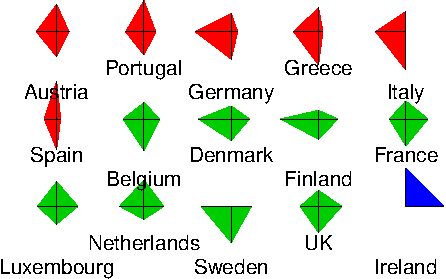
\includegraphics{sol_A1_files/figure-latex/unnamed-chunk-9-1} \end{center}

\begin{Shaded}
\begin{Highlighting}[]
\NormalTok{eupop[o,] }\OperatorTok\StringTok{ }
\StringTok{  }\KeywordTok{mutate}\NormalTok{(}\DataTypeTok{country =} \KeywordTok{rownames}\NormalTok{(.)) }\OperatorTok\StringTok{ }
\StringTok{  }\KeywordTok{gather}\NormalTok{(key, value, }\OperatorTok{-}\NormalTok{country) }\OperatorTok\StringTok{ }
\StringTok{  }\KeywordTok{ggplot}\NormalTok{(}\KeywordTok{aes}\NormalTok{(}\DataTypeTok{y =}\NormalTok{ value, }\DataTypeTok{x =}\NormalTok{ country, }\DataTypeTok{fill =}\NormalTok{ key)) }\OperatorTok{+}
\StringTok{  }\KeywordTok{geom_bar}\NormalTok{(}\DataTypeTok{stat =} \StringTok{"identity"}\NormalTok{) }\OperatorTok{+}
\StringTok{  }\KeywordTok{labs}\NormalTok{(}\DataTypeTok{x =} \StringTok{"percentage"}\NormalTok{) }\OperatorTok{+}
\StringTok{  }\KeywordTok{coord_flip}\NormalTok{() }\OperatorTok{+}
\StringTok{  }\NormalTok{ggpomological}\OperatorTok{::}\KeywordTok{scale_fill_pomological}\NormalTok{()}
\end{Highlighting}
\end{Shaded}

\begin{center}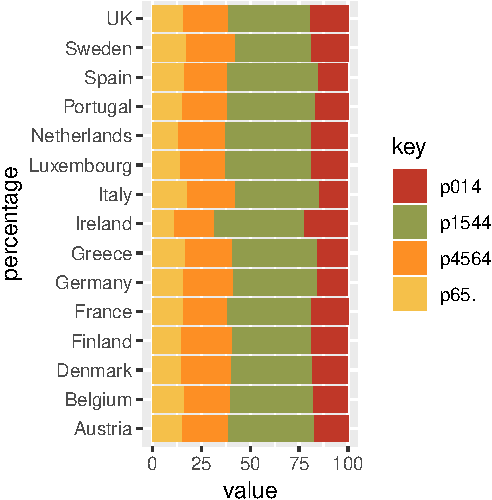
\includegraphics{sol_A1_files/figure-latex/unnamed-chunk-9-2} \end{center}

\begin{Shaded}
\begin{Highlighting}[]
\KeywordTok{library}\NormalTok{(GGally)}
\NormalTok{eupop }\OperatorTok\StringTok{ }
\StringTok{  }\KeywordTok{mutate}\NormalTok{(}\DataTypeTok{col =}\NormalTok{ clusk}\OperatorTok{+}\DecValTok{1}\NormalTok{) }\OperatorTok\StringTok{ }
\StringTok{  }\KeywordTok{ggpairs}\NormalTok{(}\KeywordTok{aes}\NormalTok{(}\DataTypeTok{colour =} \KeywordTok{factor}\NormalTok{(col), }\DataTypeTok{alpha =} \FloatTok{0.4}\NormalTok{))}
\end{Highlighting}
\end{Shaded}

\begin{center}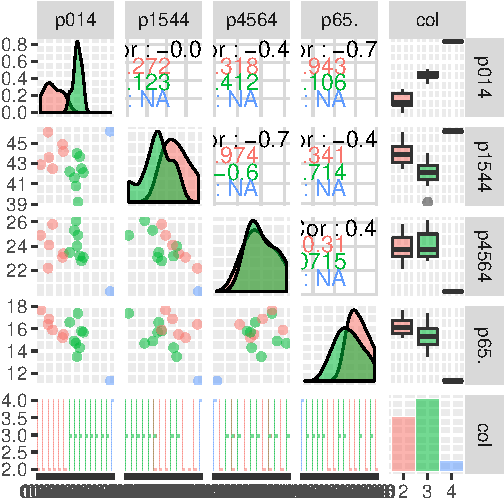
\includegraphics{sol_A1_files/figure-latex/unnamed-chunk-9-3} \end{center}

\newpage

\hypertarget{question-4}{%
\section{Question 4}\label{question-4}}

Analyzing the music data.

\begin{enumerate}
\def\labelenumi{\alph{enumi})}
\tightlist
\item
  Run the k-means algorithm over the range \(k = 1,\dots, 15\) clusters
  and record the total within cluster sum of squares (TWSS). Let nstart
  = 25. Plot k versus TWSS and choose the best fitting number of
  clusters. What do you observe? Note: remember to scale the data.
\end{enumerate}

\begin{Shaded}
\begin{Highlighting}[]
\NormalTok{music <-}\StringTok{ }\KeywordTok{read.table}\NormalTok{(}\StringTok{"data/music.txt"}\NormalTok{)}
\NormalTok{music_feat <-}\StringTok{ }\NormalTok{music }\OperatorTok\StringTok{ }
\StringTok{  }\KeywordTok{select}\NormalTok{(}\DecValTok{3}\OperatorTok{:}\DecValTok{7}\NormalTok{) }\OperatorTok\StringTok{ }\KeywordTok{mutate_all}\NormalTok{(scale)}

\NormalTok{results <-}\StringTok{ }
\StringTok{  }\KeywordTok{data.frame}\NormalTok{(}
    \DataTypeTok{tot.withinss =} \DecValTok{1}\OperatorTok{:}\DecValTok{30} \OperatorTok\StringTok{ }
\StringTok{      }\NormalTok{purrr}\OperatorTok{::}\KeywordTok{map}\NormalTok{(kmeans, }\DataTypeTok{x =}\NormalTok{ music_feat, }\DataTypeTok{nstart =} \DecValTok{25}\NormalTok{) }\OperatorTok\StringTok{ }
\StringTok{      }\NormalTok{purrr}\OperatorTok{::}\KeywordTok{map_dbl}\NormalTok{(}\StringTok{"tot.withinss"}\NormalTok{),}
    \DataTypeTok{ind =} \DecValTok{1}\OperatorTok{:}\DecValTok{30}\NormalTok{)}


\NormalTok{results }\OperatorTok\StringTok{ }
\KeywordTok{ggplot}\NormalTok{(}\KeywordTok{aes}\NormalTok{(ind, tot.withinss)) }\OperatorTok{+}
\StringTok{  }\KeywordTok{geom_line}\NormalTok{(}\DataTypeTok{colour =} \StringTok{'grey'}\NormalTok{) }\OperatorTok{+}
\StringTok{  }\KeywordTok{geom_point}\NormalTok{(}\DataTypeTok{colour =} \StringTok{"orange"}\NormalTok{, }\DataTypeTok{size =} \DecValTok{2}\NormalTok{) }\OperatorTok{+}
\StringTok{  }\KeywordTok{theme_bw}\NormalTok{() }\OperatorTok{+}
\StringTok{  }\KeywordTok{labs}\NormalTok{(}\DataTypeTok{y =} \StringTok{'TWSS'}\NormalTok{, }\DataTypeTok{x =} \StringTok{"Number of clusters"}\NormalTok{)}
\end{Highlighting}
\end{Shaded}

\begin{center}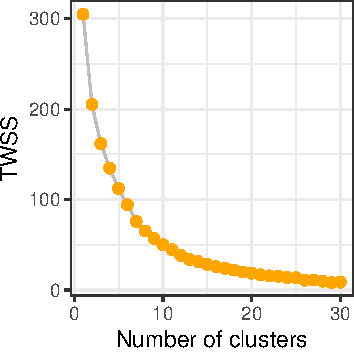
\includegraphics{sol_A1_files/figure-latex/unnamed-chunk-10-1} \end{center}

TWSS declines slowly. Data does not partition into few, small,
well-defined compact clusters

\begin{enumerate}
\def\labelenumi{\alph{enumi})}
\setcounter{enumi}{1}
\tightlist
\item
  Make a table of artist vs cluster solution from k = 5.
\end{enumerate}

\begin{Shaded}
\begin{Highlighting}[]
\NormalTok{clusk <-}\StringTok{ }\KeywordTok{kmeans}\NormalTok{(music_feat, }\DataTypeTok{centers =} \DecValTok{5}\NormalTok{, }\DataTypeTok{nstart =} \DecValTok{25}\NormalTok{)}\OperatorTok{$}\NormalTok{cluster}


\NormalTok{music }\OperatorTok\StringTok{ }
\StringTok{  }\KeywordTok{mutate}\NormalTok{(}\DataTypeTok{clusk =}\NormalTok{ clusk) }\OperatorTok\StringTok{ }
\StringTok{  }\KeywordTok{group_by}\NormalTok{(Artist, clusk) }\OperatorTok\StringTok{ }
\StringTok{  }\KeywordTok{count}\NormalTok{()}
\end{Highlighting}
\end{Shaded}

\begin{verbatim}
## # A tibble: 19 x 3
## # Groups:   Artist, clusk [19]
##    Artist    clusk     n
##    <fct>     <int> <int>
##  1 Abba          1     1
##  2 Abba          4     9
##  3 Beatles       3     8
##  4 Beatles       4     2
##  5 Beethoven     1     1
##  6 Beethoven     2     5
##  7 Beethoven     4     2
##  8 Eels          3     7
##  9 Eels          4     3
## 10 Enya          1     2
## 11 Enya          4     1
## 12 Mozart        2     6
## 13 Vivaldi       1     3
## 14 Vivaldi       2     5
## 15 Vivaldi       4     1
## 16 Vivaldi       5     1
## 17 <NA>          1     3
## 18 <NA>          2     1
## 19 <NA>          4     1
\end{verbatim}

All but one Abba tracks in a single cluster. Most of Beatles an the Eels
tracks in a single cluster.

\newpage

\hypertarget{question-5}{%
\section{Question 5}\label{question-5}}

Protein data. We want to study the similarities and differences in the
protein composition of the diets of different countries. Using any
methods that you choose from this course or otherwise, write a brief
summary.

\begin{Shaded}
\begin{Highlighting}[]
\NormalTok{protein <-}\StringTok{ }\KeywordTok{read.table}\NormalTok{(}\StringTok{"data/protein.txt"}\NormalTok{)}
\NormalTok{protein_feat <-}\StringTok{ }\NormalTok{protein }\OperatorTok\StringTok{  }\KeywordTok{select}\NormalTok{(}\DecValTok{2}\OperatorTok{:}\DecValTok{10}\NormalTok{)}
\KeywordTok{row.names}\NormalTok{(protein_feat) <-}\StringTok{ }\NormalTok{protein}\OperatorTok{$}\NormalTok{Country}
\NormalTok{d <-}\StringTok{ }\KeywordTok{dist}\NormalTok{(protein_feat)}
\NormalTok{h <-}\StringTok{ }\KeywordTok{hclust}\NormalTok{(d, }\StringTok{"complete"}\NormalTok{)}
\KeywordTok{ggdendrogram}\NormalTok{(}\KeywordTok{as.dendrogram}\NormalTok{(h))}
\end{Highlighting}
\end{Shaded}

\begin{center}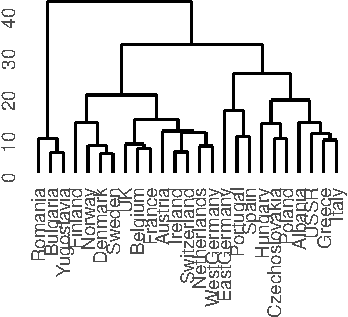
\includegraphics{sol_A1_files/figure-latex/unnamed-chunk-12-1} \end{center}

\begin{Shaded}
\begin{Highlighting}[]
\NormalTok{hc <-}\StringTok{ }\KeywordTok{cutree}\NormalTok{(h, }\DecValTok{5}\NormalTok{)}


\NormalTok{results <-}\StringTok{ }
\StringTok{  }\KeywordTok{data.frame}\NormalTok{(}
    \DataTypeTok{tot.withinss =} \DecValTok{1}\OperatorTok{:}\DecValTok{20} \OperatorTok\StringTok{ }
\StringTok{      }\NormalTok{purrr}\OperatorTok{::}\KeywordTok{map}\NormalTok{(kmeans, }\DataTypeTok{x =}\NormalTok{ protein_feat, }\DataTypeTok{nstart =} \DecValTok{10}\NormalTok{) }\OperatorTok\StringTok{ }
\StringTok{      }\NormalTok{purrr}\OperatorTok{::}\KeywordTok{map_dbl}\NormalTok{(}\StringTok{"tot.withinss"}\NormalTok{),}
    \DataTypeTok{ind =} \DecValTok{1}\OperatorTok{:}\DecValTok{20}\NormalTok{)}

\NormalTok{results }\OperatorTok\StringTok{ }
\KeywordTok{ggplot}\NormalTok{(}\KeywordTok{aes}\NormalTok{(ind, tot.withinss)) }\OperatorTok{+}
\StringTok{  }\KeywordTok{geom_line}\NormalTok{(}\DataTypeTok{colour =} \StringTok{'grey'}\NormalTok{) }\OperatorTok{+}
\StringTok{  }\KeywordTok{geom_point}\NormalTok{(}\DataTypeTok{colour =} \StringTok{"orange"}\NormalTok{, }\DataTypeTok{size =} \DecValTok{2}\NormalTok{) }\OperatorTok{+}
\StringTok{  }\KeywordTok{theme_bw}\NormalTok{() }\OperatorTok{+}
\StringTok{  }\KeywordTok{labs}\NormalTok{(}\DataTypeTok{y =} \StringTok{'TWSS'}\NormalTok{, }\DataTypeTok{x =} \StringTok{"Number of clusters"}\NormalTok{)}
\end{Highlighting}
\end{Shaded}

\begin{center}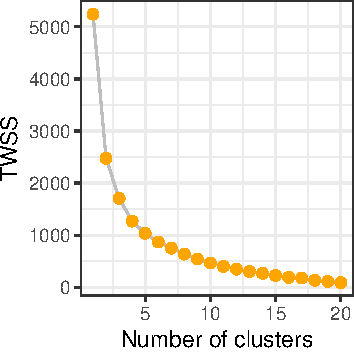
\includegraphics{sol_A1_files/figure-latex/unnamed-chunk-12-2} \end{center}

\begin{Shaded}
\begin{Highlighting}[]
\NormalTok{clusk <-}\StringTok{  }\KeywordTok{kmeans}\NormalTok{(protein_feat, }\DataTypeTok{centers =} \DecValTok{5}\NormalTok{, }\DataTypeTok{nstart =} \DecValTok{10}\NormalTok{)}\OperatorTok{$}\NormalTok{cluster}
\NormalTok{o <-}\StringTok{ }\KeywordTok{order}\NormalTok{(clusk)}
\end{Highlighting}
\end{Shaded}

\begin{Shaded}
\begin{Highlighting}[]
\KeywordTok{stars}\NormalTok{(protein_feat[o,], }\DataTypeTok{nrow =} \DecValTok{3}\NormalTok{, }\DataTypeTok{col.stars =}\NormalTok{ clusk[o]}\OperatorTok{+}\DecValTok{1}\NormalTok{)}
\end{Highlighting}
\end{Shaded}

\begin{center}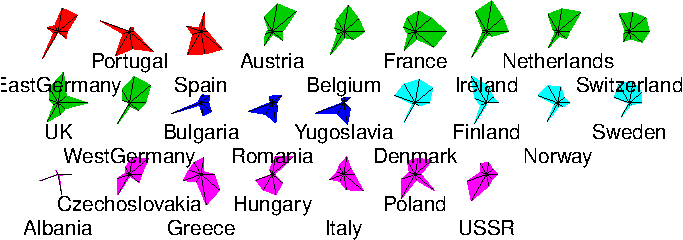
\includegraphics{sol_A1_files/figure-latex/unnamed-chunk-13-1} \end{center}

\begin{Shaded}
\begin{Highlighting}[]
\KeywordTok{table}\NormalTok{(clusk, hc)}
\end{Highlighting}
\end{Shaded}

\begin{verbatim}
##      hc
## clusk 1 2 3 4 5
##     1 0 0 0 0 3
##     2 0 8 0 0 0
##     3 0 0 3 0 0
##     4 0 0 0 4 0
##     5 7 0 0 0 0
\end{verbatim}


\end{document}
